\documentclass[serif]{beamer}
\usepackage[french]{babel}
\usepackage[T1]{fontenc}
\usepackage[utf8]{inputenc}

\usepackage{graphics} % includegraphics

\usepackage[export]{adjustbox}

\usepackage{amsmath} % align*
\usepackage{mathrsfs} % mathscr


\title{Recherche de fonctions par types}
\subtitle{Les nouvelles du front}
\date{\today}


\newcommand{\?}{\stackrel{?}{=}}


\begin{document}


\begin{frame}
  \titlepage
\end{frame}


\begin{frame}{Dessein}
  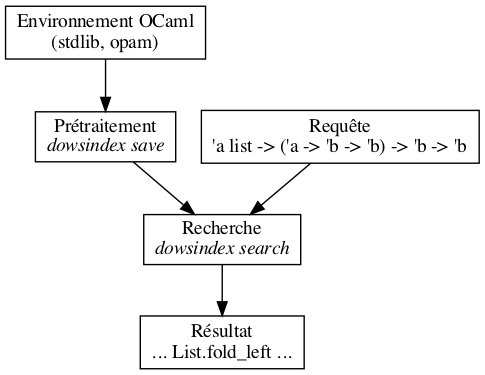
\includegraphics[scale=0.5,center]{graphs/dessein}
\end{frame}


\begin{frame}{Types à la Hindley-Milner}
  \centering
  \large
  \begin{align*}
    \mathscr V &= \{ \alpha, \beta, \gamma, \dots \} \\
    \mathscr C &= \{ (unit, 0), (int, 0), (float, 0), \dots \} \\
    \mathscr F &= \{ (list, 1), (array, 1), \dots \} \\
    \Sigma &= \mathscr C \cup \mathscr F \cup \{ (\_\!*\!\_, 2), (\_\!\rightarrow\!\_, 2) \} \\
    \mathscr T &= \mathscr T (\mathscr V, \Sigma)
  \end{align*}
  ~\\
  $int \rightarrow int \rightarrow int$ \\
  $unit * int \rightarrow int$ \\
  $(\alpha \rightarrow \beta \rightarrow \alpha) \rightarrow \alpha \rightarrow list\,(\beta) \rightarrow \alpha$
\end{frame}


\begin{frame}{Unification syntaxique}
  \centering
  \large
  $s \? t$ \\
  $\{ \sigma \,|\, \hat \sigma (s) = \hat \sigma (t) \}$ \\
  ~\\
  $\alpha * int \? list\,(float) * \beta$ \\
  $\{ \{ \alpha \mapsto list\,(float), \beta \mapsto int \} \}$ \\
  ~\\
  $\alpha * int \? \beta * list\,(float)$ \\
  $\emptyset$ \\
  ~\\
  $int \rightarrow int \rightarrow int \? int * int \rightarrow int$ \\
  $\emptyset$
\end{frame}


\begin{frame}{Isomorphisme de types linéaires}
  \large
  Ensemble $\mathscr E$ d'axiomes équationnels :
  \begin{align*}
    \alpha * \beta &\? \beta * \alpha \tag {Com-2} \\
    (\alpha * \beta) * \gamma &\? \alpha * (\beta * \gamma) \tag {Ass-2} \\
    unit * \alpha &\? \alpha \tag {Ass-0} \\
    \alpha * \beta \rightarrow \gamma &\? \alpha \rightarrow \beta \rightarrow \gamma \tag {Cur-2} \\
    unit \rightarrow \alpha &\? \alpha \tag {Cur-0}
  \end{align*}
\end{frame}


\begin{frame}{Unification sémantique}
  \textbf {Théorie équationnelle $\stackrel{\mathscr E}{=}$} \\
  Plus petite congruence par rapport à $\Sigma$ contenant $\mathscr E$ et close par substitution.
  ~\\~\\
  \centering
  $s \? t$ \\
  $\{ \sigma \,|\, \hat \sigma (s) \stackrel{\mathscr E}{=} \hat \sigma (t) \}$ \\
  ~\\
  $\alpha * int \? \beta * list\,(float)$ \\
  $\{ \{\alpha \mapsto list\,(float), \beta \mapsto int\}, \dots \}$ \\
  ~\\
  $int \rightarrow int \rightarrow int \? int * int \rightarrow int$ \\
  $\{\{\}, \dots \}$
\end{frame}


\begin{frame}{Procédure d'unification simple}
  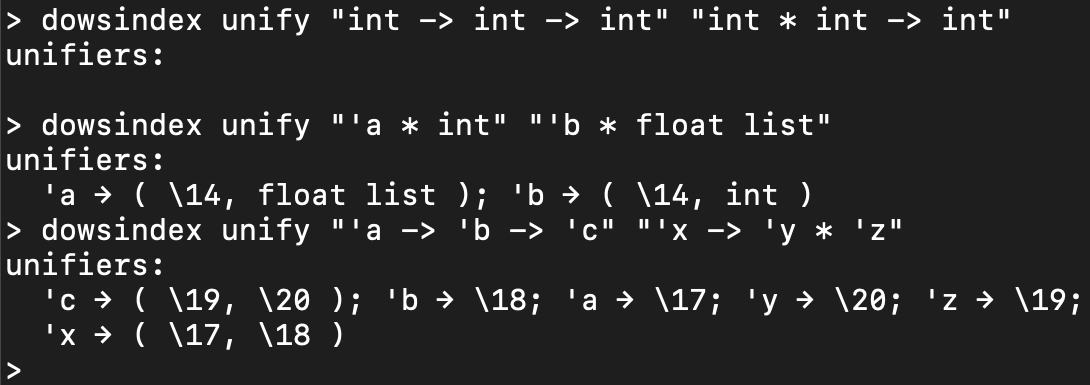
\includegraphics[scale=0.3,center]{images/unify.png}
\end{frame}


\begin{frame}{Observation 1 : nombre de variables}
  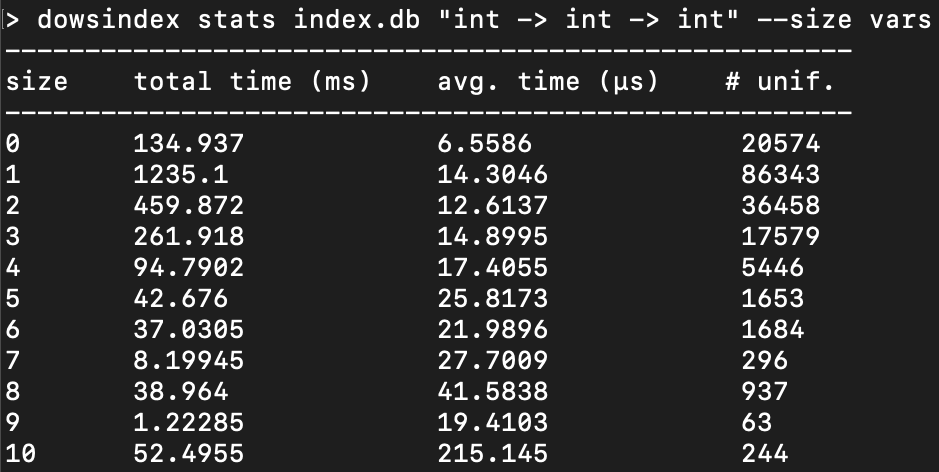
\includegraphics[scale=0.32,center]{images/stats1}
\end{frame}


\begin{frame}{Observation 2 : type en tête}
  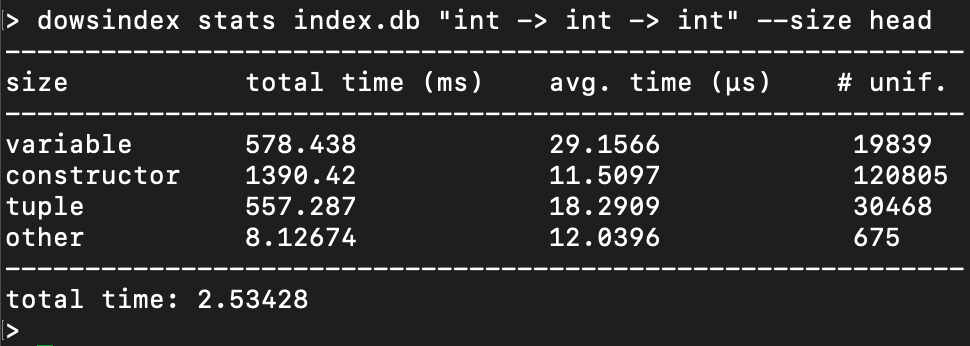
\includegraphics[scale=0.32,center]{images/stats2}
\end{frame}


\begin{frame}{Observation 3 : nombre de variables « à la racine »}
  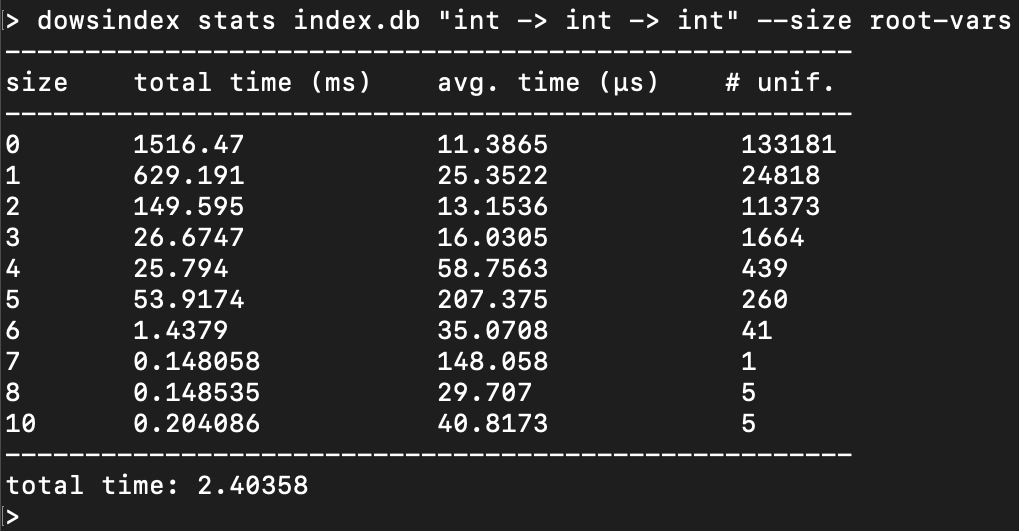
\includegraphics[scale=0.32,center]{images/stats3}
\end{frame}


\begin{frame}{Condition nécessaire 1}
  Un type dont la tête n'est pas une variable (construite avec $constr$) n'est unifiable qu'avec un type de tête soit une variable soit construite avec $constr$. \\
  ~\\~\\
  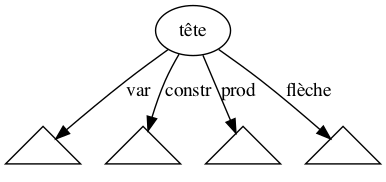
\includegraphics[scale=0.5,center]{graphs/by_head}
\end{frame}


\begin{frame}{Condition nécessaire 2}
  Un type $t$ n'admettant aucune variable « à la racine » n'est unifiable qu'avec un type :
  \begin{itemize}
    \item vérifiant le même critère et de queue de même longueur ;
    \item présentant au moins une variable « à la racine » et dont la queue est de longueur inférieure ou égale à celle de $t$.
  \end{itemize}
  ~\\
  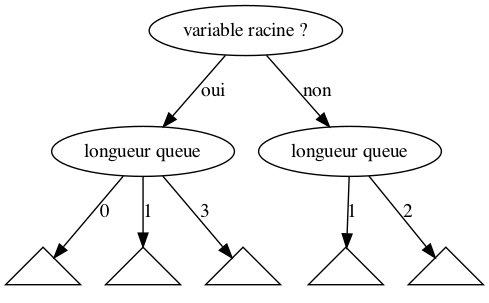
\includegraphics[scale=0.4,center]{graphs/by_tail_length}
\end{frame}


\begin{frame}{\textit {Trie} (1)}
  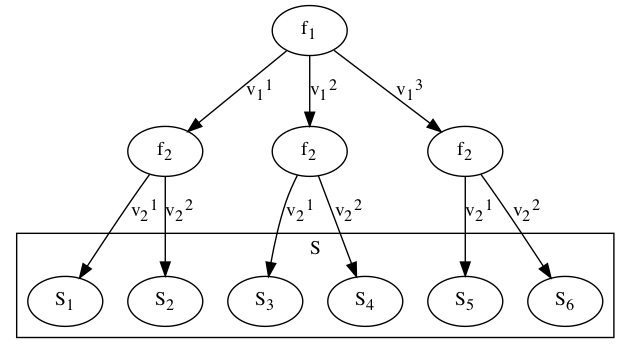
\includegraphics[scale=0.5,center]{graphs/trie1}
\end{frame}


\begin{frame}{\textit {Trie} (2)}
  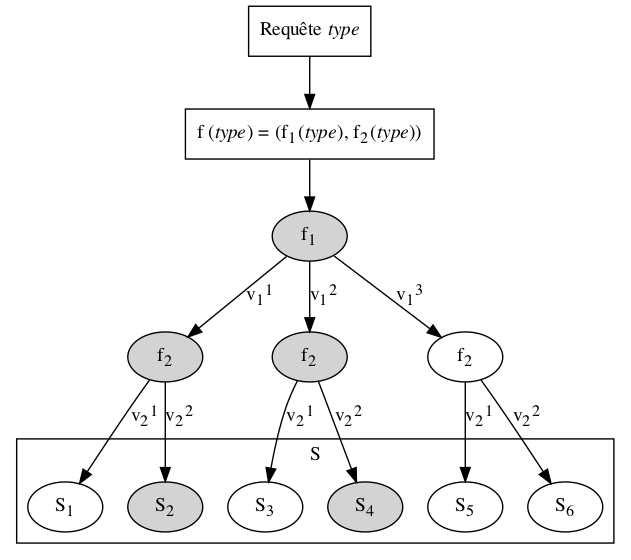
\includegraphics[scale=0.4,center]{graphs/trie2}
\end{frame}


\begin{frame}{Un bon début}
  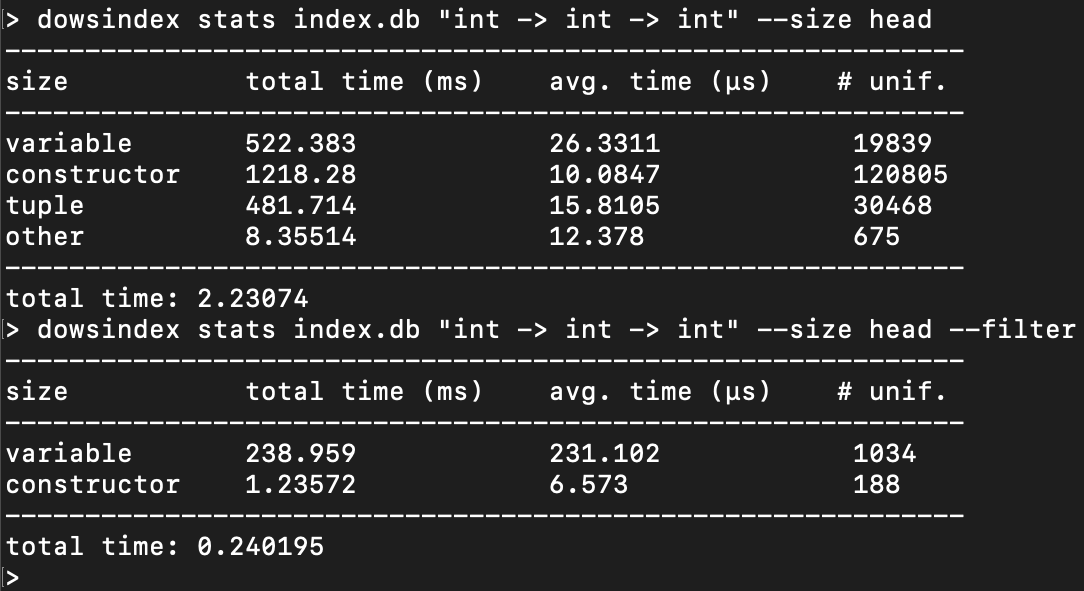
\includegraphics[scale=0.3,center]{images/stats4}
\end{frame}


\end{document}


































%%% Local Variables:
%%% mode: latex
%%% TeX-master: t
%%% End:
